\textcolor{black}{While previous generations of wireless networks were characterized by fixed radio parameters and spectrum blocks, 5G will allow utilization of any spectrum and any access technology for the best delivery of services.
\item Air-interface and RAN systems will need to be completely redesigned to accommodate a new mobile access paradigm of massive capacity, huge numbers of connections, and ultra-fast network speeds.
\item 5G will feature native support for new kinds of network deployments, including ultra-dense radio networking with self-backhauling, device- to-device communications, dynamic spectrum refarming and radio access infrastructure sharing.}\\

\section{Technologies}

% \subsection{Millimeter Waves}

\text{Every new generation of wireless network delivers faster speed and more functionality to our smart phones. 1G brought us the very first cell phones, 2G let us text for the first time, 3G brought us online, and 4G delivered the speed that we enjoy today. However, as more users come online, 4G networks have just about reached their limit at a time when users want even more data for their smart phones and devices. Now we are headed towards 5G, the next generation of wireless. 5G will be able to handle 1000 times more traffic than today’s networks and it will be up to 10 times faster than 4G LTE. Simply imagine downloading an HD movie in under a second, and then let your imagination run wild with what might be possible. 5G will be the foundation for virtual reality, autonomous driving, the internet of things, and things we cannot even imagine. What exactly is a 5G network? The truth is, experts cannot tell us what 5G actually is because they do not even know yet. Right now, there are a few brands already out there. This research will be considering five brand technologies emerging as a foundation of 5G.}\\

\begin{figure}
    \centering
    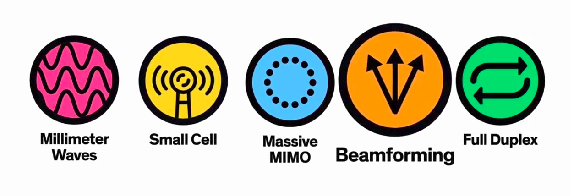
\includegraphics[width=10cm]{Images/now.png}
    \caption{Technologies}
    \label{fig:my_label}
\end{figure}

\subsection{Millimeter Waves}

\subsubsection{Introduction}

\text{{Studies on the fifth generation (5G) wireless communication system are gaining more momentum worldwide in an attempt to provide solutions for the exponential increase of mobile data traffic by 2020. Although 5G is in its embryonic stage, some trends have appeared on how to design 5G networks, such as to make it green and soft, as proposed by China Mobile. Multiple research topics have been identified as 5G candidates, including large-scale antenna systems (LSAS), non-orthogonal multiplex access, full duplex, spectrum sharing, high-frequency bands (e.g., millimeter-wave, mm Wave), high-density networks, new network architecture, new wave-form design, and so on. These technologies may have great potential in system performance improvement in 5G.}}\\

\subsection{Reference Signal Design}\\

\text{Smart phones and other electronic devices in your home use very specific frequencies on the radio frequency spectrum, typically those under 6 GHz but these frequencies are starting to get more crowded as carriers can only squeeze so many bits of data on the same amount of radio frequency spectrum. As more devices come online, we are going to start seeing slower service and more dropped connections. The solution is to open up some new real estage, so most of the companies such as Huawei are experimenting with broadcasting on shorter millimeter waves. Those that fall between 30 and 300 GHz of spectrum have never been used before for mobile devices and opening it up means more bandwidth for everyone. However, there is a catch: millimeter waves cannot travel well through buildings or other obstacles and tend to be absorbed by plants and rain. To avoid this problem, small cell networks can be used.}\\

\section{Small Cell}
Small cell networks: today’s wireless networks rely on tall high-powered cell towers to broadcast their signals over long distances, but we should keep in mind high-frequency millimeter waves have a harder time traveling through obstacles. This means that if we move behind an obstacle, we lose our signal. Small cell networks can solve this problem by using thousands of low-power mini base stations. These base stations would be much closer together than traditional towers, forming a sort of relay team to transmit signals around obstacles. This technology would be especially useful in cities, as the user moved behind an obstacle his smart phone would automatically switch to a new base station in better range of his device, allowing him to keep his connection.

\section{Full Duplex}
Full duplex: back in the day we used a wall gataki and in order for us to communicate using this technology, we had to take turns taking and listening. Today’s cellular base stations have that exact same hold-up as basic antennas can only do one job at a time either transmit or receive. This is because of a principle called reciprocity which is the decency for radio waves to travel both forward and backward along the same frequency. To understand this, it helps to think of waves like a train loaded up with data. The frequency is traveling on a train track, but if there is a second train trying to go in the opposite direction on the same track you are going to get some interference. Until now, the solution has been to have the trains take turns, or to put all the trains on different tracks or frequencies but this can be made a lot more efficient by working around reciprocity. Other researchers have used silicon transistors to create high speed switches that halt the backward role of these waves. It is like a signaling system that can momentarily reroute the trains so that they can get past each other. This means there is a lot more traffic on each track, and everything is a whole lot faster.
% MIMO most stands for multiple-input multiple-output, today’s 4G base stationshave about a dozen ports for antennas that handle all cellular traffic but massive MIMO base stations can support about a hundred ports this could increase the capacity of toda’s networks by a factor of 22 or more accurent with the experts massive MIMO comes with its own complications today’s cellular antennas broadcast information in every direction at once and all of those crossing signals could cause serious interference, which is one of the reason why 5G jumped the next tecnology above.\\

\section{Beam forming }
Beam forming is more precisely like a traffic signaling system for cellular signals instead of broadcasting in every direction. It would allow a base station to send a focus stream of data to a specific user. This precision prevents interferences and is way more efficient. This means stations could handle more incoming and outgoing data streams at once. In this research, it is explained how it works as well. If we are in a cluster building and you try to make a phone call, your signal is ricocheting off of surrounding buildings and crisscrossing with other signals from users in the area. A massive MIMO (multiple-inlet multiple-outlet, more on this is the next paragraph) base station receives all of these signals and keeps track of the timing and the direction of their arrival. It then uses signal processing algorithms to triangulate exactly where each signal is coming from and plots the best transmission route back through the air to each phone. Sometimes it will even bounce individual packets of data in different directions off of buildings or other objects to keep signals from interfering with each other, the result is a coherent data stream sent only to \\

\begin{figure}[t]
    \centering
    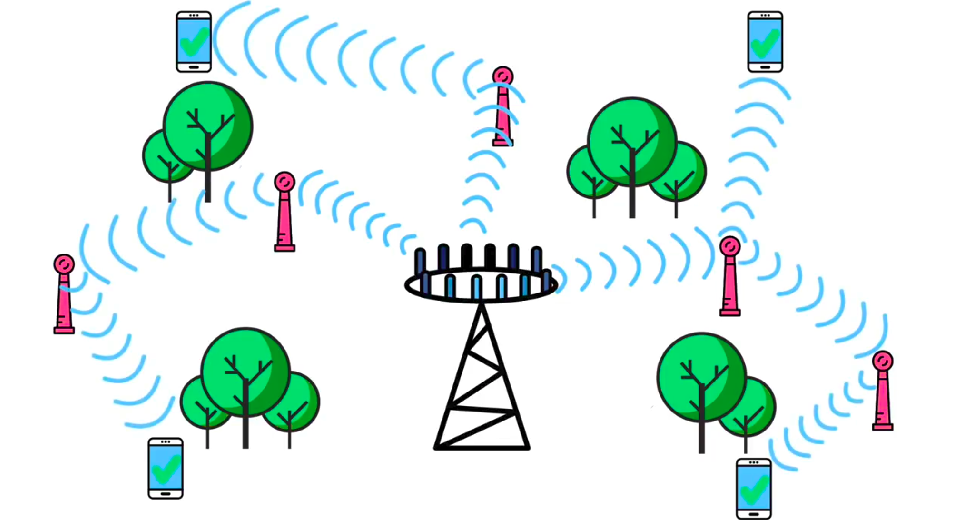
\includegraphics[width=9cm]{Images/small-cell.png}
    \caption{Small Cell}
    \label{fig:my_label}
\end{figure}

\begin{figure}
    \centering
    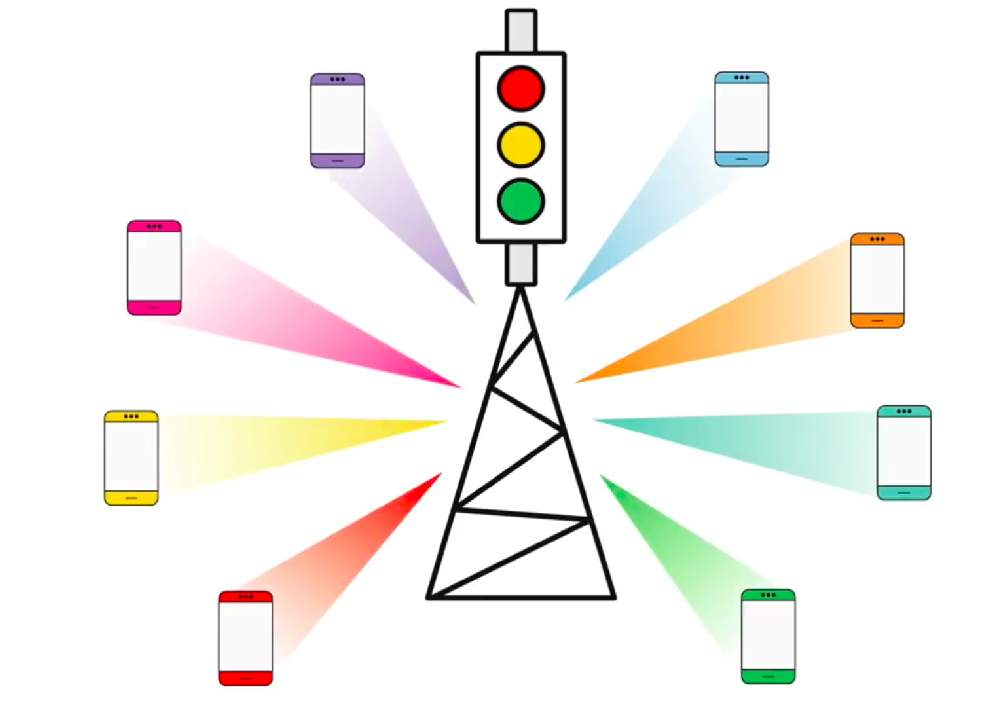
\includegraphics[width=8cm]{Images/Massive.png}
    \caption{Full-duplex}
    \label{fig:my_label}
\end{figure}\\

\section{Massive MIMO}
MIMO stands for Multiple-Input Multiple-Output. Today’s 4G base stations have about a dozen ports for antennas that handle all cellular traffic, but massive MIMO base stations can support about a hundred ports. This could increase the capacity of today’s networks by a factor of 22 or more. Currently, according to experts massive MIMO comes with its own complications. Today’s cellular antennas broadcast information in every direction at once and all of those crossing signals could cause serious interference, which is one of the reasons why 5G jumped to the next technology which will be discussed in further paragraphs..\\
